\section{The Setting: Taiwan's SME Economy and the Kingdom of Screws}\label{sec:setting}

Taiwan runs on small business. The Ministry of Economic Affairs counts
\textbf{1.716 million} small and medium enterprises --- 98.87\% of all firms ---
employing \textbf{9.19 million people}, or 79.3\% of the workforce\cite{moea}.
That headline number is often used to dramatize the carbon problem (``1.71
million SMEs must decarbonize''). This proposal refuses that framing: most of
those firms are shops and services with no carbon obligation at all. The honest
picture is one of \emph{concentration} --- shown in Figure~\ref{fig:funnel}.

\begin{figure}[htbp]
\centering
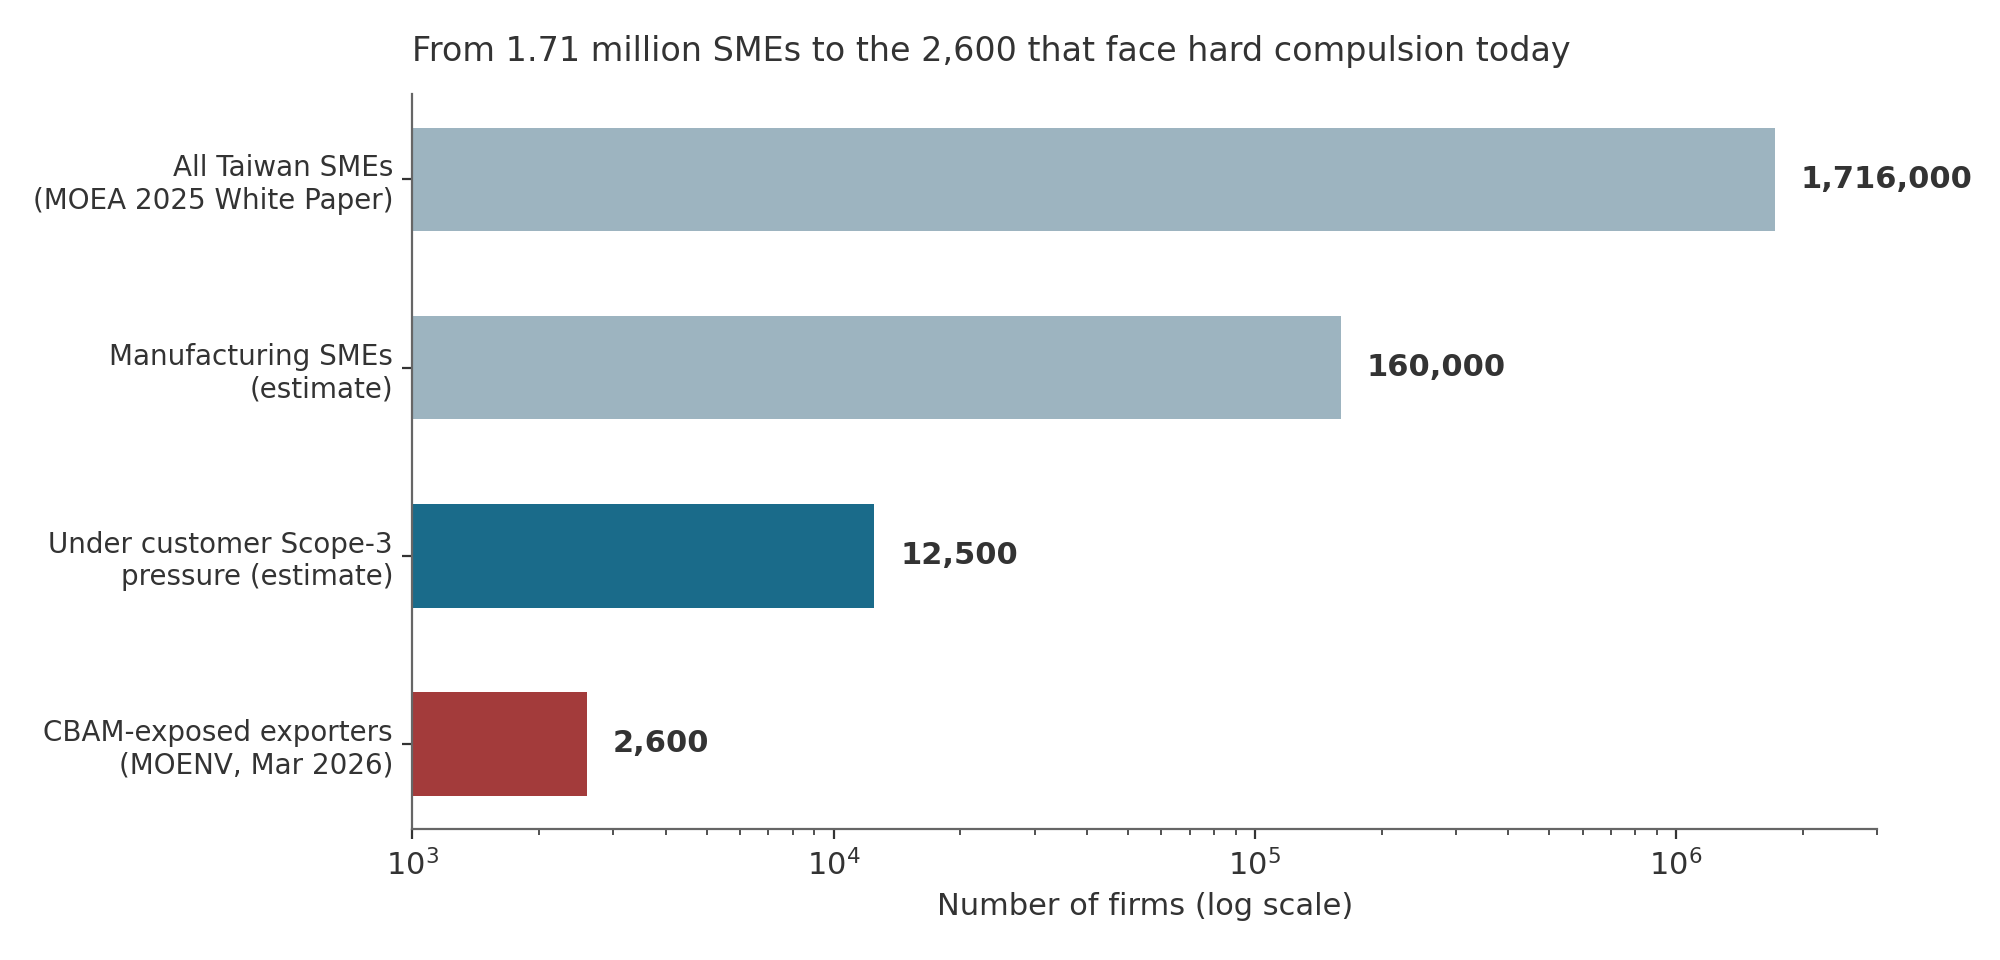
\includegraphics[width=0.95\textwidth]{chart1_funnel.png}
\caption[From 1.71 million SMEs to 2,600 firms under hard compulsion]{Narrowing
from all Taiwanese SMEs to the population under hard compulsion. The 1,716,000
and 2,600 figures are official (MOEA\cite{moea}; MOENV\cite{tpt-cbam}); the two
middle bars are this proposal's estimates.}
\label{fig:funnel}
\end{figure}

The 2,600 firms at the sharp end are concentrated in one place and one product.
The Gangshan--Luzhu district of Kaohsiung --- nicknamed the \textbf{``Kingdom
of Screws''} --- hosts roughly \textbf{1,800 fastener manufacturers}, about 700
of them organized under the Taiwan Industrial Fasteners
Institute\cite{goebel,ktimes}. Their global standing is out of all proportion
to their size (Figure~\ref{fig:sector}, Table~\ref{tab:sector}).

\begin{figure}[htbp]
\centering
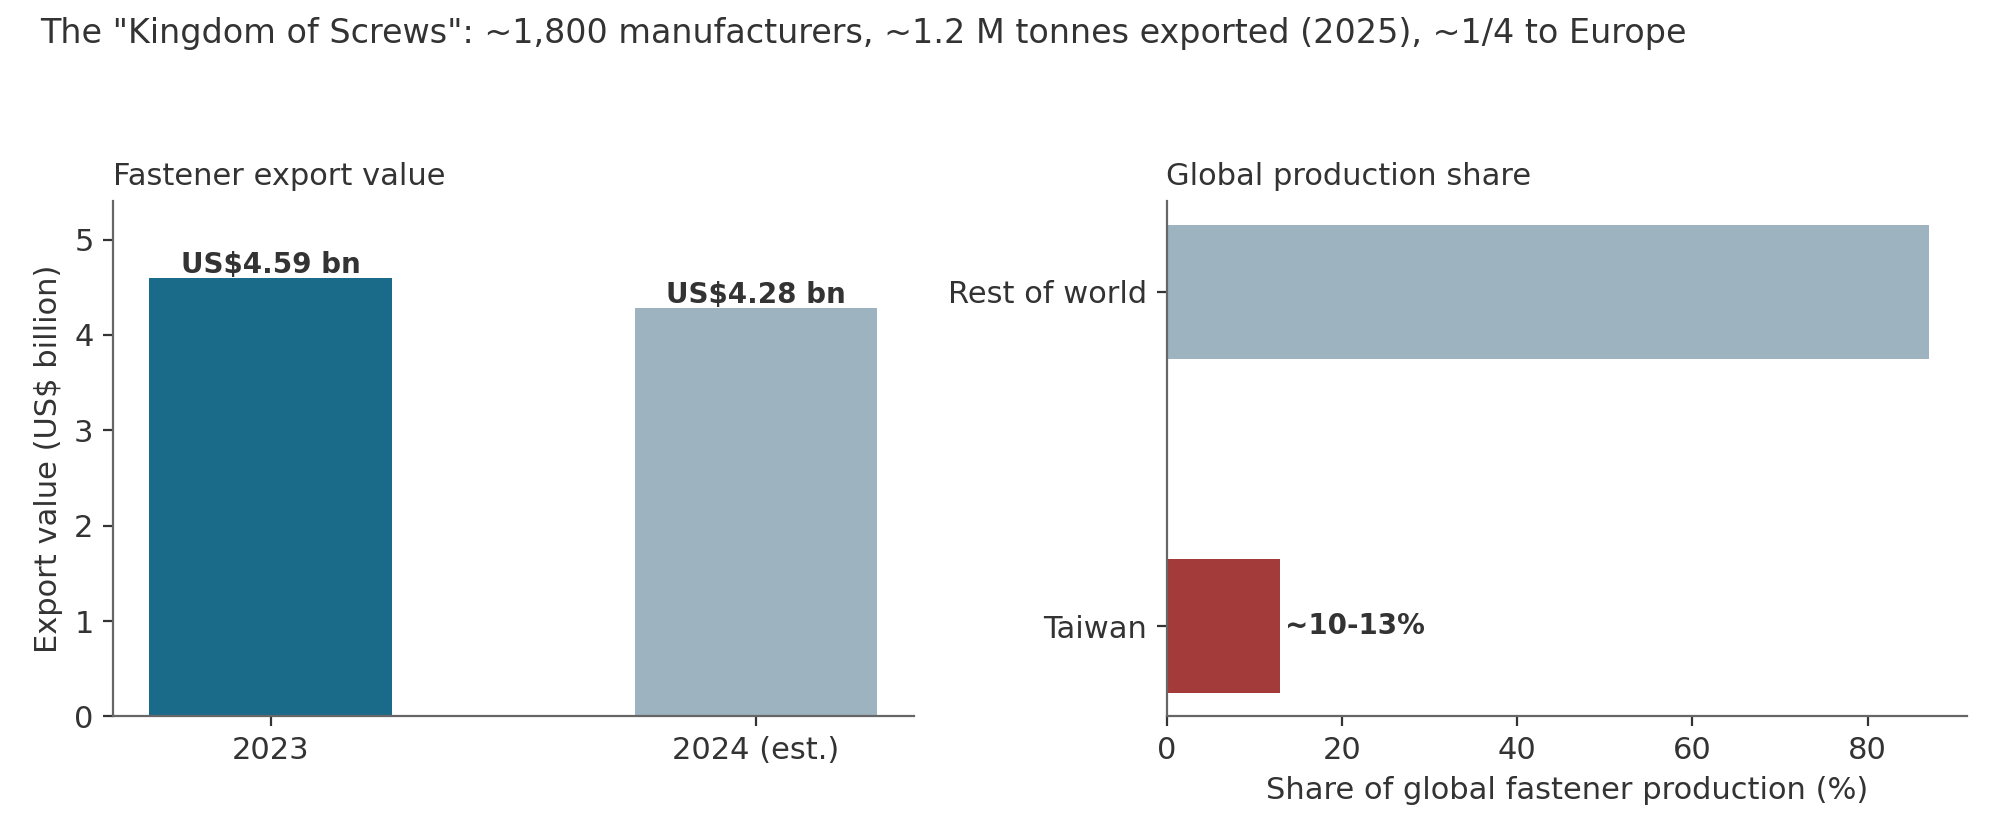
\includegraphics[width=0.95\textwidth]{chart5_sector.png}
\caption[Fastener sector snapshot: export value and world share]{Sector
snapshot: export value (left, industry statistics\cite{fwexport}) and share of
world production (right\cite{ktimes,goebel}).}
\label{fig:sector}
\end{figure}

\begin{table}[htbp]
\caption{The Taiwanese fastener sector at a glance}
\label{tab:sector}
\small
\begin{tabularx}{\textwidth}{@{}p{0.3\textwidth}Xp{0.21\textwidth}@{}}
\toprule
\textbf{Indicator} & \textbf{Value} & \textbf{Source, date} \\
\midrule
Global rank & Top-3 exporter (\#2 by value in 2023 reporting; \#3 by volume in 2025--26 reporting) & CW 2023\cite{cw}; KT 2026\cite{ktimes} \\
Share of world production & $\sim$10--13\% & \cite{ktimes,goebel} \\
Export volume & $\sim$1.2 million tonnes (2025) & \cite{ktimes} \\
Export value & US\$4.59\,bn (2023); $\sim$US\$4.28\,bn (2024 est.) & Fastener World\cite{fwexport} \\
Share destined for Europe & $\sim$one quarter & \cite{cw} \\
Number of manufacturers & $\sim$1,800 (mostly SMEs; TIFI $\sim$700 members) & \cite{goebel} \\
Typical firm structure & Family-run; nationally 51.79\% of SMEs are sole proprietorships / family firms; 58.22\% older than 8 years & MOEA\cite{moea} \\
Embedded emissions & $\sim$2 tCO$_2$e per tonne of fasteners (industry estimate) & \cite{specialinsert} \\
\bottomrule
\end{tabularx}
\end{table}

\textbf{Economically}, these are ``hidden champions'': firms with
aerospace-grade precision supplying European automakers, administered by family
members on spreadsheets, with aging workforces and no in-house data or ESG
staff. \textbf{Environmentally}, fastener-making is steel plus electricity plus
heat --- wire drawing, cold forging, thread rolling, heat treatment,
electroplating --- drawn from a grid that emitted \textbf{0.474~kgCO$_2$e per
kWh in 2024}\cite{moeaea}, high by European standards. The SME controls neither
the grid nor the steel mill. What it \emph{could} control --- proving its actual
numbers instead of being assigned worst-case ones, and running its flexible
loads at cleaner, cheaper hours --- is precisely what it has no tools for.
